\chapter{Some Background}\label{chap:background}

\minitoc % comment this line to hide this chapter's TOC

\begin{quote}
{\it This chapter provides a thorough background on the topic of the thesis. The literature on this particular topic is huge, but we will try our best.}
\end{quote}

%----------------------------------------------------------
% Introduction
%----------------------------------------------------------
\section{Introduction}\label{chap:background:introduction}

The topic of this thesis is very challenging, so we need to provide sufficient background information.

\begin{figure}[!h] 
	\centering
	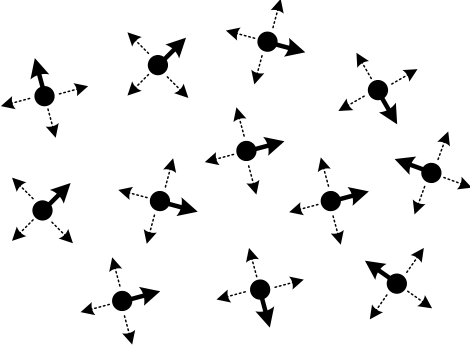
\includegraphics[scale=0.7]{images/fig01.png}
	%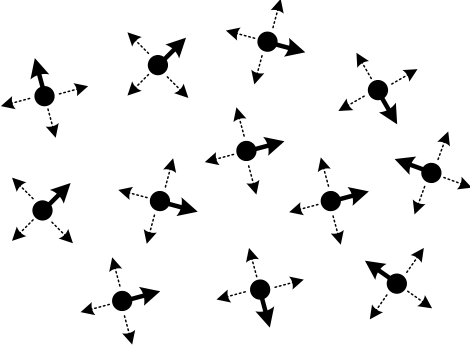
\includegraphics[width=0.5\textwidth]{images/fig01.png}
	\caption{Some random figure}
	\label{fig:background:random}
\end{figure}

%----------------------------------------------------------
% Summary
%----------------------------------------------------------
\section{Summary}\label{chap:background:summary}
This concludes this chapter
